\section{Introduction}
    As technology becomes more advanced, those who design, use, and are affected by it in other ways want to know that it will perform correctly, and understand why it does what is does, and how to use it appropriately. In essence, people who interact with advanced technology want to be able to trust it appropriately, and then act on that trust.

    In interpersonal relationships, and otherwise, humans act largely based on trust. For example, a supervisor asks a subordinate to accomplish a task based on several factors that indicate they can trust them to accomplish that task. When consumers make purchases, they do so with trust that the product will perform as promised. Likewise, when using something like an autonomous vehicle, the user must be able to trust it appropriately in order to use it properly.

    With the rapid advancement of the capabilities of intelligent computing technology to do tasks that were previously assumed to be too complicated for computers, there has been much recent discussion regarding how humans can trust this technology -- although the connection to trust is not always made explicit, per se. This discussion has taken place both in public \cite{Spectrum2016-jv,DeSteno2014-cq,Cranz2017-yh,Cassel2017-tn,Danks2017-sb}, business \cite{Banavar2016-nm, Khosravi2016-ke,Moody2017-vd,Rudnitsky2017-in,Benioff2016-tc}, and academic \cite{Groom2007-bz,Lloyd2014-bb,Goodrum_2016-fm,Foley2017-qj,Ghahramani2015-yq,Castelvecchi2016-mr} settings.

    Those who discuss \emph{how} to trust a specific technology are really referring to the need for some indication of the appropriate level of trust to give said technology. In other words, it is desirable to \emph{design} capabilities and methods for intelligent technology which help us achieve appropriate levels of trust in that technology. These capabilities and methods are collectively referred to as \emph{assurances}. %%
    
    Specifically, this survey investigates what assurances an Artificially Intelligent Agent (AIA) can provide to a human user in order to affect their trust. The colloquial definitions of `appropriate use', `assurance', `AIA', and `trust' should suffice for now to give the reader a general idea of the motivation; more formal definitions will be presented in section \ref{sec:background}. It is the author's position that there are many researchers, from different disciplines, who will potentially be interested in this work. This group includes those who are interested in working with, trusting, interpreting, understanding, and/or regulating AIAs.

    Figure \ref{fig:SimpleTrust_one_way} is a simple diagram of the trust cycle that exists between a human user and an AIA (justification for the existence of this cycle will be presented later). Simply, the user's trust is affected by assurances that in turn affect the user's behaviors in interacting with the AIA (e.g. to trust AIA with responsibilities, or not). To fully understand and appreciate the importance of assurances, one must have a more formal understanding of each component in figure \ref{fig:SimpleTrust_one_way}. %This is because the cycle is serial, and cannot be complete with any of the components missing. 
    This paper provides an overview of the components of figure \ref{fig:SimpleTrust_one_way}. It then turns a more focused attention to assurances, and investigates some of the related research that has been done to date. From this survey of literature, properties and classifications of assurances are created, and directions and considerations for further research are presented.

    \begin{figure}
        \centering
        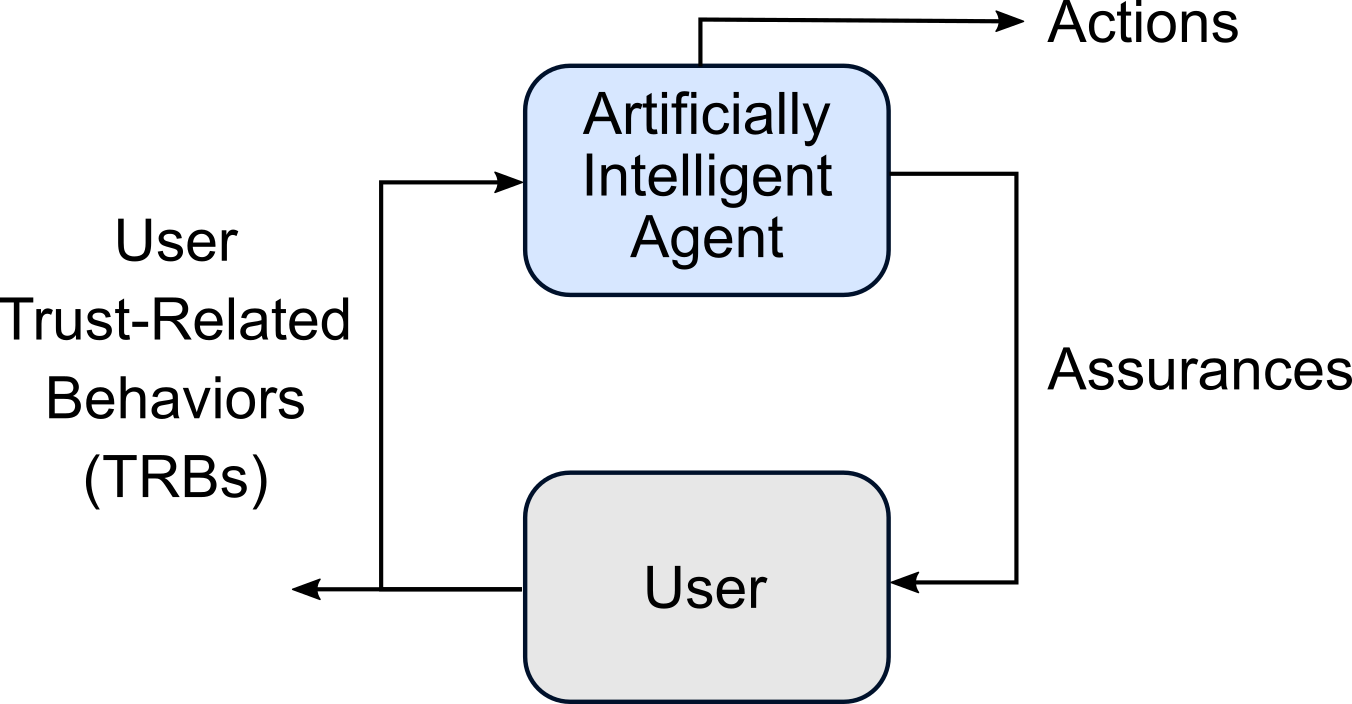
\includegraphics[width=0.7\textwidth]{Figures/SimpleTrust_one_way.png}
        \caption{Diagram depicting the simple one-way trust development relationship between a human user and an AIA. Based on a user's level of trust they take certain actions (e.g. give AIA commands), these commands can lead the AIA to certain actions and/or to provide assurances to the user in order to affect their trust.}
        \label{fig:SimpleTrust_one_way}
    \end{figure}

    Some of the novel contributions of this paper include: a detailed description and definition of assurances in general human-AIA relationships; an argument that trust-related behaviors should be used to measure the effect of assurances on user trust; presenting the idea that assurances can be either explicit or implicit; suggestions for promising research directions for explicit assurances. To this end, section \ref{sec:background} provides definitions for each of the terms. In section \ref{sec:methodology} we discuss the methodology used when compiling this survey. Afterwards, section \ref{sec:survey} will discuss the current landscape of assurances that exist in the literature. Section \ref{sec:discussion} discusses some important insights into the classification and design of assurances. Finally, section \ref{sec:conclusions} contains some last discussion and conclusions.
